\documentclass[11pt]{scrartcl}
\usepackage{dominatrix}
\usepackage{solarized-light}
\lstset{
language=python
}

\renewcommand\thesection{Problem \arabic{section}}
\renewcommand\thesubsection{\arabic{section} (\alph{subsection})}
\renewcommand\thesubsubsection{(\roman{subsubsection})}

\newcommand{\mearth}{M_{\bigodot}}

\DeclareMathOperator{\AU}{AU}
\DeclareMathOperator{\arcsec}{arcsec}
\DeclareMathOperator{\pc}{pc}
\DeclareMathOperator{\km}{km}
\DeclareMathOperator{\m}{m}
\DeclareMathOperator{\cm}{cm}
\DeclareMathOperator{\rad}{rad}
\DeclareMathOperator{\s}{s}
\DeclareMathOperator{\degrees}{degrees}
\DeclareMathOperator{\degree}{degree}
\DeclareMathOperator{\arcmin}{arcmin}
\DeclareMathOperator{\parsec}{parsec}
\DeclareMathOperator{\lightyears}{light-years}
\DeclareMathOperator{\yr}{yr}


\newcommand\pow[2]{\ensuremath{#1 \times 10^{#2}}}

\title{Problem Set 2}
\subject{ASTR 1404 Stars, Galaxies, and Cosmology}
%\author{James H. Applgate}
\begin{document}
\maketitle

The law of skinny triangles may be written 

\[a = \theta D\]

with $a$, $D$ in the same distance units and $\theta$ in radians. The definition of the parsec allows us to write it in the form

\[a(\AU) = \theta(\arcsec) \cdot D (\parsec)\]

The definition of a parsec, a length of $1\AU$ subtends an angle of $\arcsec$ if viewed from a distance of $1 \parsec$, is clearly expressed by this relation.

\section{More Skinny Triangle}

\subsection{}

The distance to the binary is

\[D(\parsec) = \frac{a(\AU)}{\theta(\arcsec)} = \frac{1}{0.1} = 10\parsec\]

Here $a = 1\AU$ is the Earth-Sun distance and $\theta$ is the parallax, $\theta = 0.1\arcsec$. The skinny triangle is:

\begin{figure}[H]
\centering
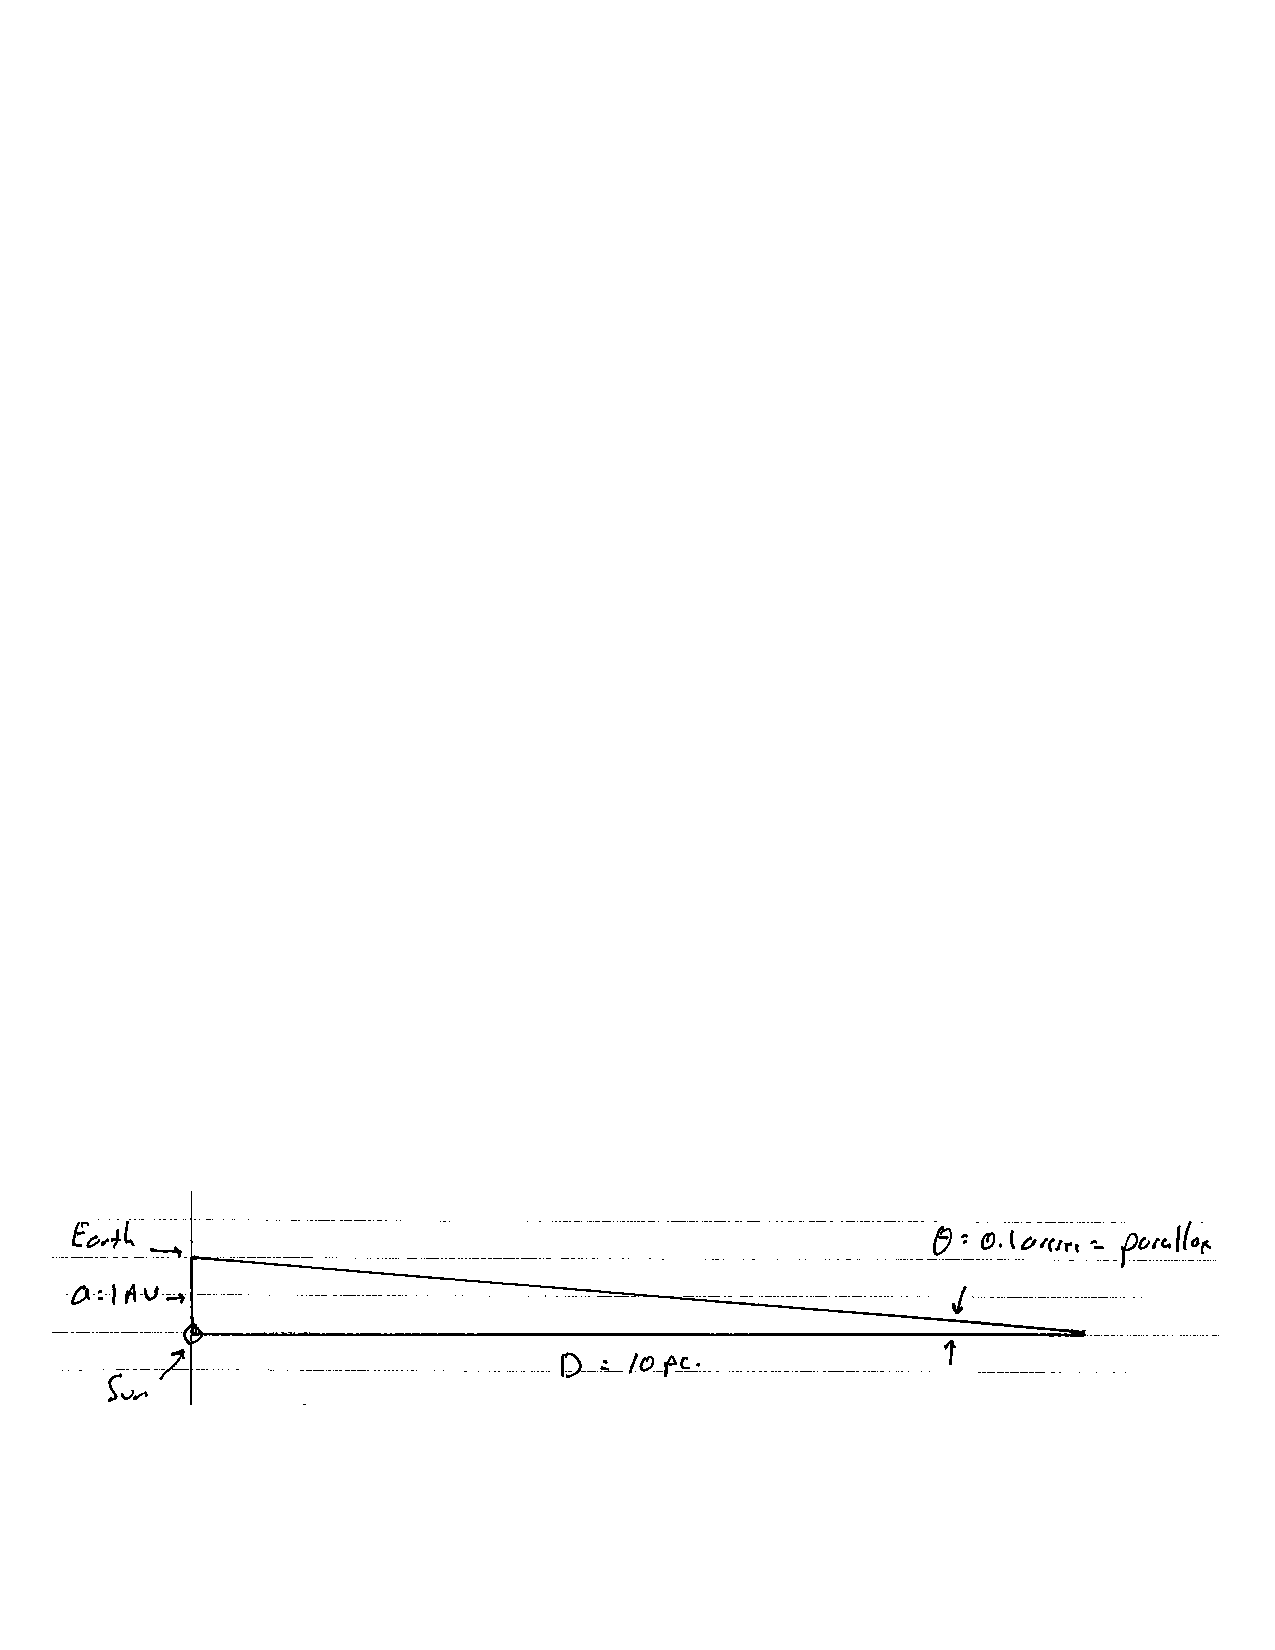
\includegraphics[width=\textwidth]{figures/problem-set-2-earth-binary-1.pdf}
\caption{Skinny triangle of Earth-Sun and the binary.}
\end{figure}

If this seems easy, it is. This ease is why the $\parsec$ is defined the way it is.

\subsection{}

\begin{figure}[H]
\centering
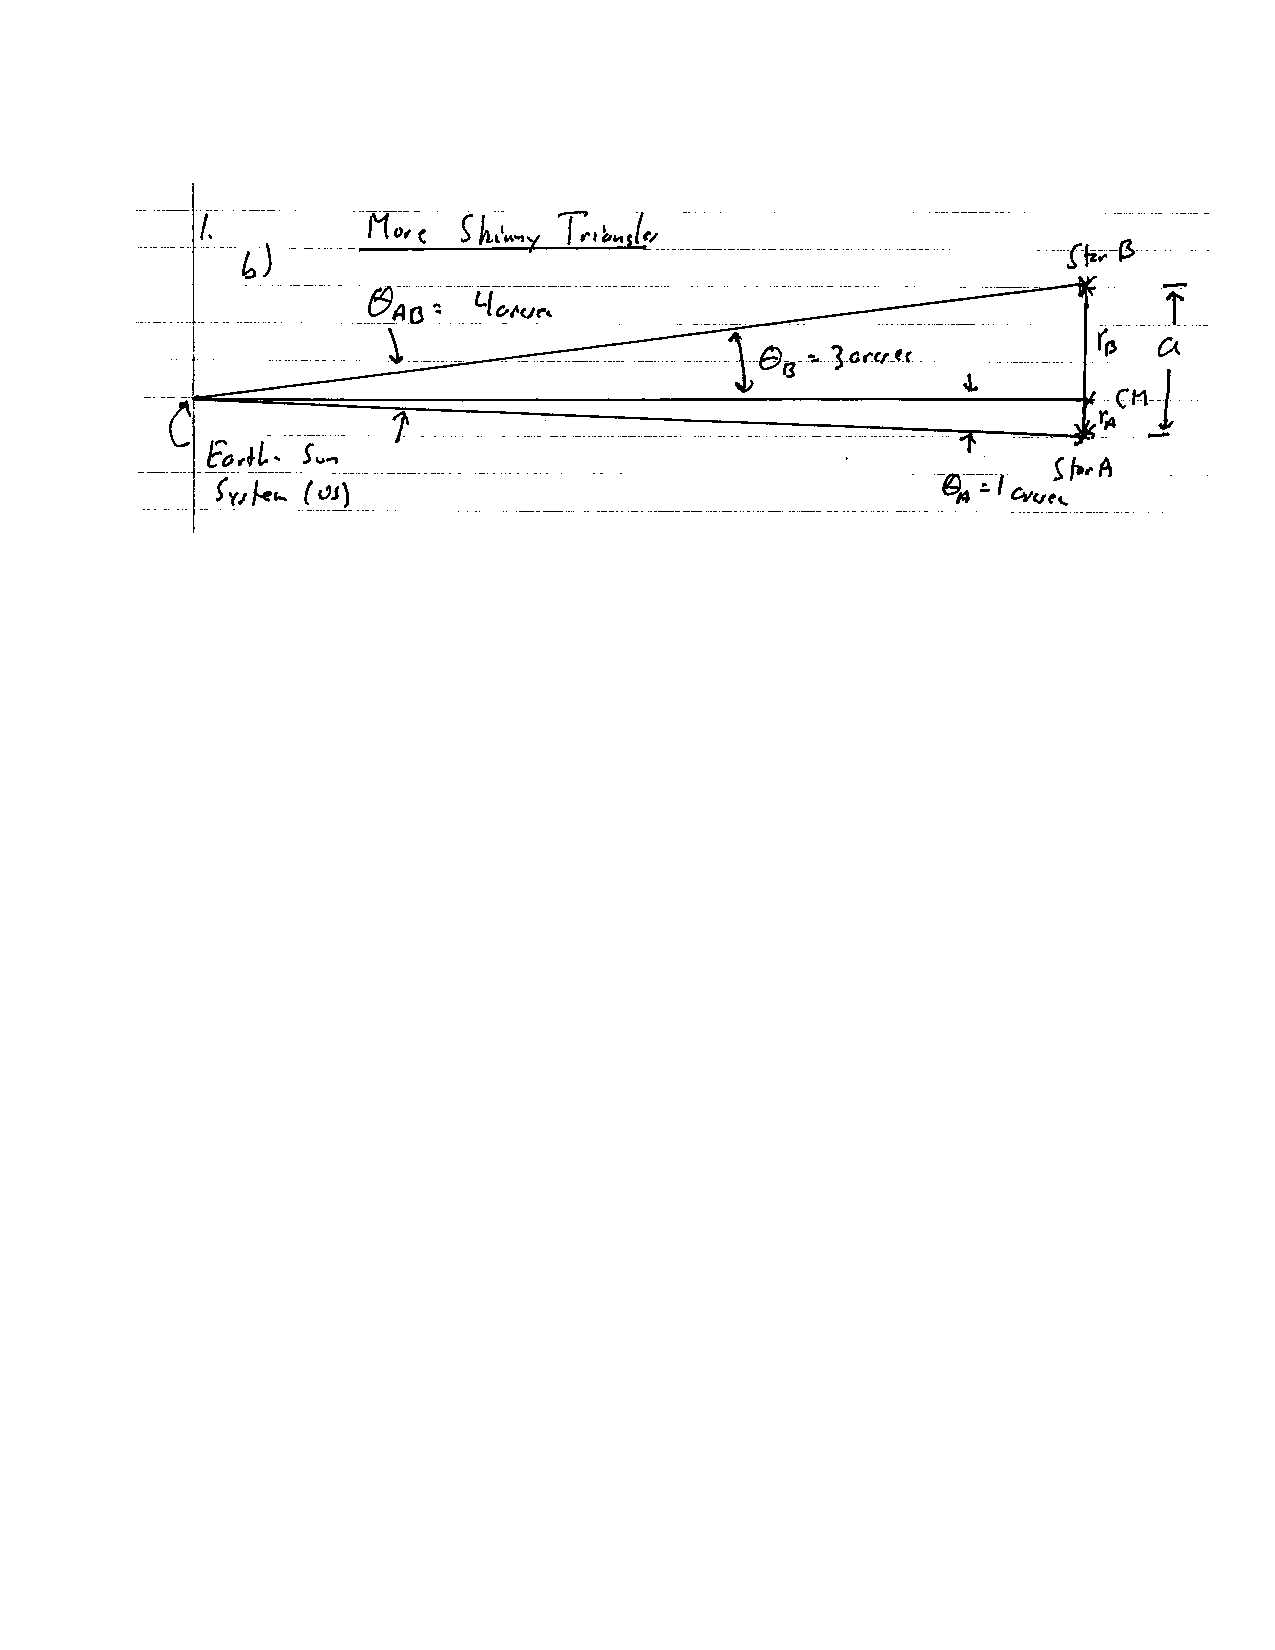
\includegraphics[width=\textwidth]{figures/problem-set-2-earth-binary-2.pdf}
\caption{Skinny triangle of Earth-Sun and the binary.}
\end{figure}

The physical separation in $\AU$ is given by:

\[a(\AU) = \theta(\arcsec) \cdot D(\parsec)\]

with

\begin{align*}
&D = 10 \parsec = \text{Distance to Binary} \\
&\theta = \theta_{AB} = 4\arcsec = \text{Separation between Star A and Start B} \\
&a(\AU) = 4 * 10 = 40 \AU = \text{Physical separation between Star A and Star B}
\end{align*}

\subsection{}

Kepler's Third Law may be written:

\[p^2(\yr) = \frac{a^2(\AU)}{M_T(M_{\mearth})}\]

where $P(\yr)$ is the orbital period in years, $a(\AU)$ is the separator in $\AU$, and $M_T = M_A + M_B$ is the total mass in $\mearth$. This gives:

\[M_T = \frac{a^3(\AU)}{p^2(\yr)} = \frac{40^3}{100^2}\mearth = 6.4 \mearth\]

\subsection{}

The teeter-totter law (definition of the center of mass) is

\[M_A r_A = M_Br_B\]

with

\[r_A + r_B = a\]

\[M_A + M_B = M_T\]

A bit of algebra produces the result:

\[M_A = \frac{r_B}{a} M_T\]

\[M_B = \frac{r_A}{a} M_T\]

The law of skinny triangles gives ($D = \text{Distance to Binary}$)

\[a = \theta_{AB} \cdot D\]

\[r_A = \theta_{A} \cdot D\]

\[r_B = \theta_{B} \cdot D\]

Hence,

\[M_A = \frac{r_B}{a} M_T = \frac{\theta_B}{\theta_{AB}}M_T\]

\[M_B = \frac{r_A}{a}M_T = \frac{\theta_A}{\theta_{AB}}M_T\]

The masses $M_A$ and $M_B$ are:

\[M_A = \frac{3}{4} M_T = \frac{3}{4} 6.4 \mearth = 4.8 \mearth\]

\[M_B = \frac{1}{4} M_T = \frac{1}{4} 6.4 \mearth = 1.6\mearth\]

Note that $\theta_A = 1 \arcsec$, $\theta_B = 3 \arcsec$, $\theta_{AB} = 4 \arcsec$.

\section{Alpha Centauri}

\subsection{}

\[D(\parsec) = \frac{1}{\text{parallax in arcsec}} = \frac{1}{0.752} = 1.33\parsec\]

\subsection{}

Recall that $a(\AU) = \theta(\arcsec) * D(\parsec)$. We know that $\theta = \theta_{AB} = 17.6 \arcsec$. Then,

\[a(\AU) = 17.6 * 1.33 = 23.4 \AU\]

\subsection{}

Recall that $p^2(\yr) = \frac{a^3(\AU)}{M_T(\mearth)}$. Then,

\[M_T(\mearth) = \frac{a^3(\AU)}{p^2(\yr)} = \frac{23.4^3}{80.1^2} = 2.00\mearth\]

\subsection{}

\[A = M(\alpha\text{CenA}) = \frac{\theta_B}{\theta_{AB}}M_T = \frac{9.7}{17.6}M_T = 1.10\mearth\]

\[A = M(\alpha\text{CenB}) = \frac{\theta_A}{\theta_{AB}}M_T = \frac{7.9}{17.6}M_T = 0.90\mearth\]


\section{Procyon}

\subsection{}

Given that the parallax of Procyon is $0.29 \parsec$, the distance $D$ is

\[D = \frac{1}{0.29} = 3.45\parsec\]

\subsection{}

The separation $a$ is

\[a = \theta_{AB}D = 4.5 * 3.45 = 15.5\AU\]

\subsection{}

The total mass $M_T$ is

\[M_T = \frac{a^3(\AU)}{p^2(\yr)}\mearth = \frac{15.5^3}{40.6^2} = 2.27\mearth]\]

\subsection{}

\[M_A = \frac{\theta_B}{\theta_{AB}} M_T = \frac{3.3}{4.5} (2.27)\mearth = 1.66\mearth\]

\[M_A = \frac{\theta_A}{\theta_{AB}} M_T = \frac{1.2}{4.5} (2.27)\mearth = 0.61\mearth\]





\end{document}
